% =====================================================================
% DRAFT — formalization pearl. Format-agnostic (acmart/LIPIcs later).
% Style goals: technical but plain; story-driven (each section opens with a
% question and travels to its answer); every claim argued; humility throughout;
% scope stated exactly (the Socratic anti-fissure rules are honoured verbatim).
% =====================================================================
\documentclass[11pt]{article}
\usepackage{amsmath,amssymb,amsthm,booktabs,graphicx,hyperref}
\usepackage[table]{xcolor}
\definecolor{ggteal}{HTML}{1B6F8C}
\definecolor{ggband}{HTML}{DCE7EB}
\definecolor{ggamber}{HTML}{E08A1E}
\usepackage[margin=1in]{geometry}
\graphicspath{{figures/}}
\newtheorem{theorem}{Theorem}
\newtheorem{lemma}{Lemma}
\newtheorem{definition}{Definition}
\newcommand{\lean}[1]{\texttt{#1}}
\newcommand{\Z}{\mathbb{Z}}
\newcommand{\R}{\mathbb{R}}

\title{\bf Random Signs into Matchings\\[3pt]
  \large\normalfont A Godsil--Gutman identity, formalized in Lean~4}
\author{Carles Mar\'in\thanks{The Lean formalization was carried out with Claude (Anthropic) as an AI research instrument; all design decisions, mathematics, and claims are the author's responsibility.}\\[3pt]
  \normalsize Independent researcher\\
  \normalsize \texttt{karlesmarin@gmail.com}}
\date{June 2026}

\begin{document}
\maketitle

\begin{abstract}
I report a machine-checked formalization, in Lean~4 / Mathlib, of the
Godsil--Gutman identity: the average characteristic polynomial of a uniformly
random $\pm1$ signing of a graph is its \emph{matching polynomial}.
Along the way I formalize the matching polynomial itself and its deletion
recurrence---to my knowledge, the first such development in any proof
assistant. I then isolate the one ingredient that makes the proof work, a
$\Z/2$ \emph{sign-averaging} fact ($\sum_{s=\pm1}s^{k}=2\,[k\text{ even}]$), and
show that the \emph{same} formal lemma underlies a second, moment-level
identity (the parity-closed-walk count of Chen--van~Dam--Bu). Finally I
formalize the Bilu--Linial spectral decomposition of a signed $2$-lift, the
bridge that connects all of this to Ramanujan graphs.
I am deliberately precise about what is and is not done: the headline
theorems are \lean{sorry}-free and depend only on the three standard axioms,
but the deep half of the Marcus--Spielman--Srivastava program
(Heilmann--Lieb real-rootedness, interlacing families) is mapped, not
formalized. This is a pearl, not a landmark; I hope it is a useful first
stone.
\end{abstract}

% ---------------------------------------------------------------
\section{A question about signings}
\label{sec:intro}

Take a finite graph $G$ and put a sign, $+1$ or $-1$, on each edge. The
resulting \emph{signed adjacency matrix} $A_s$ has a characteristic polynomial
$\det(xI-A_s)$. Different signings give different polynomials. A natural
question---and the starting point of a beautiful chapter of spectral graph
theory---is:
\begin{quote}\itshape
  what do you get if you average $\det(xI-A_s)$ over all $2^{|E|}$ signings?
\end{quote}
The answer, due to Godsil and Gutman~\cite{GodsilGutman1981}, is striking: the
average is exactly the \emph{matching polynomial}
$\mu_G(x)=\sum_k(-1)^k m_k\,x^{n-2k}$, where $m_k$ counts the $k$-edge matchings
of $G$ (Figure~\ref{fig:gg}). A spectral average over random signs equals a
purely combinatorial count of matchings.

\begin{figure}[t]
  \centering
  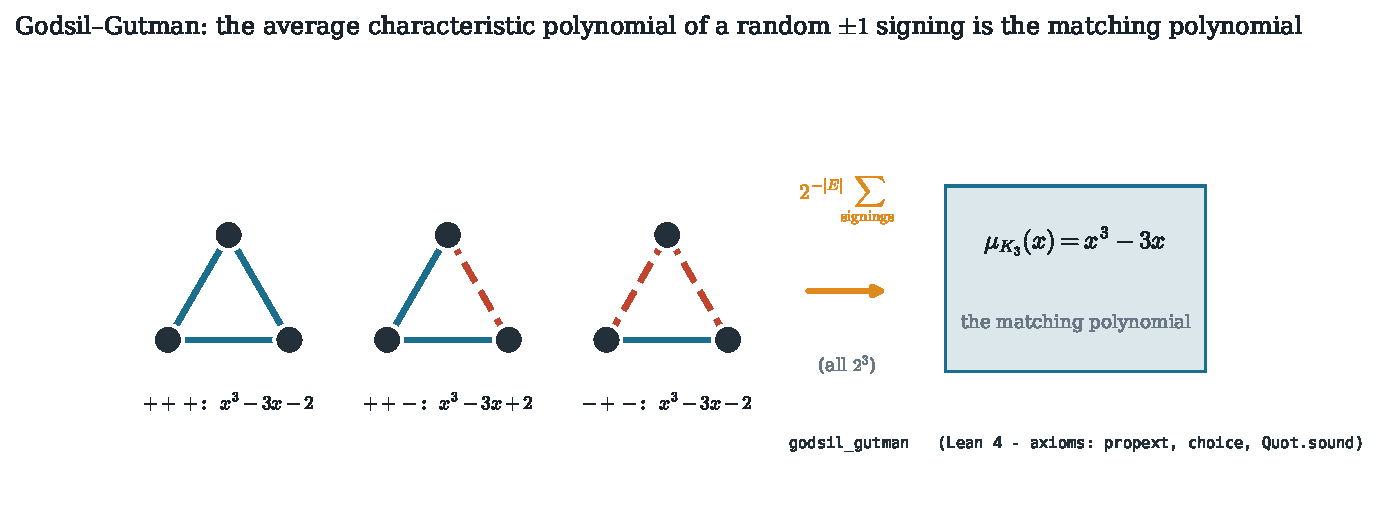
\includegraphics[width=\textwidth]{fig1_godsil_gutman.pdf}
  \caption{Godsil--Gutman on $K_3$: each $\pm1$ signing (teal $+$, dashed red
  $-$) gives a characteristic polynomial; their average is the matching
  polynomial $\mu_{K_3}(x)=x^3-3x$. Machine-checked as \lean{godsil\_gutman}.}
  \label{fig:gg}
\end{figure}

Why should anyone outside spectral graph theory care, and why formalize it?
Two reasons travel together through this paper.

\paragraph{It is the door to Ramanujan graphs.}
A signing of $G$ is the same data as a $2$-lift (double cover) of $G$, and the
``new'' eigenvalues of the lift are precisely the eigenvalues of $A_s$
(Bilu--Linial; Section~\ref{sec:twolift}). So the average characteristic
polynomial of the new eigenvalues is $\mu_G$. Heilmann and
Lieb~\cite{HeilmannLieb1972} proved that the roots of $\mu_G$ all lie in
$[-2\sqrt{\Delta-1},\,2\sqrt{\Delta-1}]$---the Ramanujan threshold
(Figure~\ref{fig:bound}). Marcus, Spielman and
Srivastava~\cite{MSS2015a} then used an interlacing-families argument to show
that \emph{some} signing achieves a lift whose new eigenvalues are all within
that threshold, proving the existence of Ramanujan graphs of every degree.
Godsil--Gutman is the first link of that chain.

\begin{figure}[t]
  \centering
  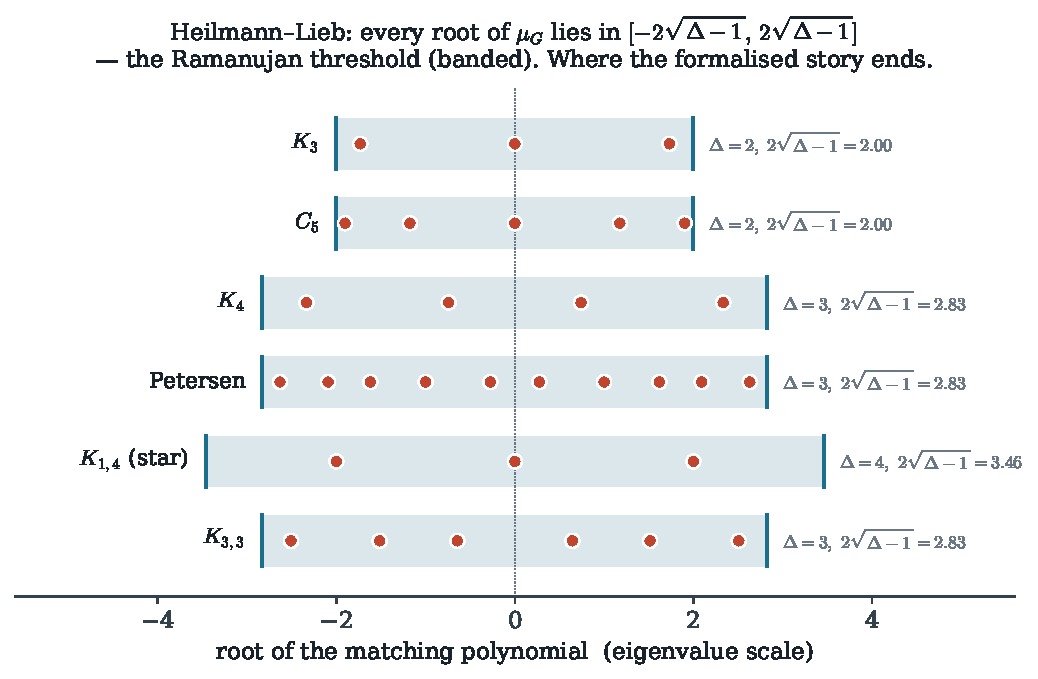
\includegraphics[width=\textwidth]{fig2_ramanujan_bound.pdf}
  \caption{Heilmann--Lieb: the (computed) roots of the matching polynomial all
  lie inside the band $[-2\sqrt{\Delta-1},\,2\sqrt{\Delta-1}]$, the Ramanujan
  threshold. This bound is the endpoint of the program; here it is mapped
  (Section~\ref{sec:future}), not yet formalized.}
  \label{fig:bound}
\end{figure}

\paragraph{It hides a single, reusable pattern.}
The proof of Godsil--Gutman, when one looks closely, rests on one tiny fact:
averaging a sign monomial over $\pm1$ kills every odd power and doubles every
even one. This is a $\Z/2$ Fourier projection, and---this is the part I found
worth telling---the \emph{same} formal lemma drives an apparently different,
moment-level identity (Section~\ref{sec:engine}). Formalization makes such
shared structure not a slogan but something a reader can check by name.

\paragraph{Contributions.}
I contribute, all in Lean~4 / Mathlib and all \lean{sorry}-free with
\lean{\#print axioms} reporting only \lean{propext}, \lean{Classical.choice},
\lean{Quot.sound} (Table~\ref{tab:results}):
\begin{enumerate}\itemsep2pt
\item the matching polynomial, the matching number, and the deletion
  recurrence $m_{k+1}(G)=m_{k+1}(G{-}v)+\sum_{u\sim v}m_k(G{-}v{-}u)$;
\item a complete proof of the Godsil--Gutman identity (\lean{godsil\_gutman});
\item the $\Z/2$ sign-averaging engine and its two consumers---Godsil--Gutman
  at the characteristic-polynomial level and the parity-closed-walk kernel at
  the moment level;
\item the Bilu--Linial $2$-lift charpoly factorization
  (\lean{charpoly\_twoLift}).
\end{enumerate}
I am equally explicit about the boundary of the work
(Section~\ref{sec:future}): Heilmann--Lieb and the interlacing-families step are
mapped in detail but not formalized.

% Professional tables for the formalization-pearl paper.
% Requires \usepackage{booktabs,amsmath,amssymb} and \usepackage[table]{xcolor}
% in the main preamble, plus colors ggteal / ggband defined there.

% ---------- Table 1: formalised results ----------
\begin{table}[t]
  \centering
  \small
  \arrayrulecolor{ggteal}
  \caption{The formalised results (Lean~4 / Mathlib). All theorems are
  \texttt{sorry}-free and non-vacuous; \texttt{\#print axioms} reports only
  \texttt{propext}, \texttt{Classical.choice}, \texttt{Quot.sound}.}
  \label{tab:results}
  \begin{tabular}{@{}llc@{}}
    \toprule
    \rowcolor{ggteal}
    \textcolor{white}{\textbf{Lean name}} & \textcolor{white}{\textbf{Statement}} & \textcolor{white}{\textbf{Status}} \\
    \midrule
    \rowcolor{ggband}
    \texttt{godsil\_gutman} & $\sum_{\mathrm{cfg}}\det(xI-A_{\mathrm{cfg}})=\#\mathrm{cfg}\cdot\mu_G$ & proven \\
    \texttt{matchingPoly} (+infra) & $\mu_G=\sum_k(-1)^k m_k\,x^{n-2k}$ (no prior formalization found) & defined \\
    \rowcolor{ggband}
    \texttt{matchingNumber\_recurrence} & $m_{k+1}(G)=m_{k+1}(G{-}v)+\sum_{u\sim v} m_k(G{-}v{-}u)$ & proven \\
    \texttt{charpoly\_twoLift} & $\det\!\bigl(xI-\bigl[\begin{smallmatrix}B&C\\C&B\end{smallmatrix}\bigr]\bigr)=\mu_{B+C}\,\mu_{B-C}$ & proven \\
    \rowcolor{ggband}
    \texttt{signAvg\_ne\_zero\_iff} & sign-monomial survives $\iff$ multiplicities even & proven \\
    \texttt{sum\_signOf\_prod\_pow} & $\mathbb{Z}/2$ parity-projection kernel (moment level) & proven \\
    \midrule
    \emph{Heilmann--Lieb} & $\mathrm{roots}(\mu_G)\subseteq[-2\sqrt{\Delta-1},\,2\sqrt{\Delta-1}]$ & future \\
    \rowcolor{ggband}
    \emph{interlacing families} & $\exists$ signing with $\lambda_{\max}\le\lambda_{\max}(\overline{\,\cdot\,})$ & future \\
    \bottomrule
  \end{tabular}
  \arrayrulecolor{black}
\end{table}

% ---------- Table 2: numerical cross-checks ----------
\begin{table}[t]
  \centering
  \small
  \arrayrulecolor{ggteal}
  \caption{Numerical cross-checks of the formalised identities (SymPy, exact).
  Left: the average characteristic polynomial of all $\pm1$ signings equals
  $\mu_G$ (Godsil--Gutman). Right: the average $d$-th spectral moment equals the
  number of parity-closed walks (here $d=4$).}
  \label{tab:checks}
  \begin{tabular}{@{}llcc@{}}
    \toprule
    \rowcolor{ggteal}
    \textcolor{white}{\textbf{$G$}} & \textcolor{white}{\textbf{$2^{-|E|}\!\sum_{\mathrm{signings}}\det(xI-A_s)$}} & \textcolor{white}{\textbf{$=\mu_G$?}} & \textcolor{white}{\textbf{$\overline{\mathrm{tr}(A_s^{4})}=P_4$}} \\
    \midrule
    \rowcolor{ggband}
    $K_3$ & $x^{3}-3x$         & $\checkmark$ & $18$ \\
    $C_4$ & $x^{4}-4x^{2}+2$   & $\checkmark$ & $24$ \\
    \rowcolor{ggband}
    $C_5$ & $x^{5}-5x^{3}+5x$  & $\checkmark$ & $30$ \\
    $K_4$ & $x^{4}-6x^{2}+3$   & $\checkmark$ & $60$ \\
    \rowcolor{ggband}
    $K_{3,3}$ & $x^{6}-9x^{4}+18x^{2}-6$ & $\checkmark$ & $90$ \\
    Petersen & $x^{10}-15x^{8}+75x^{6}-145x^{4}+90x^{2}-6$ & $\checkmark$ & $150$ \\
    \bottomrule
  \end{tabular}
  \arrayrulecolor{black}
\end{table}


% ---------------------------------------------------------------
\section{What exactly is being averaged?}
\label{sec:setting}

Before a machine can check anything, the objects must be pinned down. I work
over an arbitrary finite vertex type $V$.

\begin{definition}[Signed adjacency]
A signing is a function $\mathrm{cfg}\colon \mathrm{Sym2}\,V\to\mathrm{Bool}$ on
unordered pairs. The signed adjacency matrix $A_{\mathrm{cfg}}$ is the symmetric
real matrix that is $\pm1$ on edges (according to $\mathrm{cfg}$) and $0$
elsewhere.
\end{definition}

A small but honest subtlety surfaces immediately, and it is worth stating
plainly rather than hiding it. I let $\mathrm{cfg}$ range over \emph{all}
unordered pairs, not only edges; the non-edge bits are simply ignored by
$A_{\mathrm{cfg}}$. Consequently each genuine signing is counted
$2^{|\mathrm{Sym2}\,V|-|E|}$ times, and my theorem reads
\[
  \boxed{\;\sum_{\mathrm{cfg}}\det(xI-A_{\mathrm{cfg}})
  \;=\;\bigl(\#\mathrm{cfg}\bigr)\cdot \mu_G\;},
  \qquad \#\mathrm{cfg}=2^{|\mathrm{Sym2}\,V|}.
\]
Dividing by $\#\mathrm{cfg}$ recovers the textbook edge-average
$2^{-|E|}\sum_{\text{signings}}=\mu_G$ exactly; the redundant non-edge bits
cancel. I chose the all-pairs phrasing because it makes the proof's
$\Z/2$-Fourier structure (Section~\ref{sec:engine}) uniform over the whole
index type, at the cost of this one bookkeeping remark.

\begin{definition}[Matching polynomial]
$\mu_G(x)=\sum_{k=0}^{\lfloor n/2\rfloor}(-1)^k m_k(G)\,x^{\,n-2k}$, where
$m_k(G)$ is the number of $k$-subsets of edges that are pairwise
vertex-disjoint and $n=|V|$.
\end{definition}

Mathlib has a rich theory of simple graphs and of characteristic polynomials,
but no matching polynomial; building it (and proving its deletion recurrence)
was a prerequisite, and is, to my knowledge, the first such infrastructure in
a proof assistant.

% ---------------------------------------------------------------
\section{How a machine proves Godsil--Gutman}
\label{sec:gg}

The classical one-paragraph proof expands $\det(xI-A_{\mathrm{cfg}})$ over
permutations, sums over signings, and observes that only permutations that are
\emph{involutions made of edges}---that is, matchings---survive. Turning that
paragraph into a checked proof meant making each ``observe that'' explicit.
The architecture is a short pipeline; I sketch it and flag the two places that
fought back.

\paragraph{Only edge-involutions survive.}
Writing the determinant as $\sum_{\sigma}\mathrm{sign}(\sigma)\prod_i(\cdots)$
and summing over signings, the contribution of a permutation $\sigma$ is, up to
sign and a power of $x$, an inner sum over signings of a product along
$\sigma$'s support. I prove (\lean{innerSum\_eq\_ite}) that this inner sum is
$\#\mathrm{cfg}$ when $\sigma$ is an edge-involution ($\sigma^2=1$ with every
$2$-cycle an edge) and $0$ otherwise. The ``$0$ otherwise'' is exactly the
$\Z/2$ cancellation: a permutation with a non-paired edge contributes a sign
that averages away.

\paragraph{Edge-involutions are matchings.}
The surviving permutations biject with matchings: an edge-involution
$\sigma$ maps to its set of $2$-cycle edges, and a matching maps back to the
involution that swaps each edge's endpoints. I build this bijection
explicitly---\lean{matchingOfPerm} one way, \lean{permOfMatching} the other---
and prove both round-trips. A pleasant surprise was that the inverse map is
\emph{proof-irrelevant} in the matching hypothesis (the permutation's data
depends only on the matching, not on the proof that it is one), which let the
\lean{Finset.sum\_bij'} obligations discharge cleanly.

\paragraph{The two hard spots.}
First, a coercion: casting $(-1)^k$ from the unit group $\Z^\times$ through
$\Z$ into $\R[x]$. The natural Mathlib rewrite
(\lean{Units.val\_pow\_eq\_pow\_val}) is definitionally a no-op and silently
fails to rewrite; I needed a short induction
(\lean{intCast\_units\_neg\_one\_pow}). Second, the final reassembly required a
fibered sum over matching size with a boundary term, handled with
\lean{Finset.sum\_fiberwise\_of\_maps\_to} and the matching-size bound
$2k\le n$. Neither is deep, but both are the kind of friction a formalization
must absorb and a paper should be honest about.

The result, \lean{godsil\_gutman}, is the precise statement of
Section~\ref{sec:setting}, machine-checked.

% ---------------------------------------------------------------
\section{The engine underneath: one $\Z/2$ fact, two identities}
\label{sec:engine}

Why does the cancellation in Section~\ref{sec:gg} happen? Because of a single
arithmetic fact about signs:
\[
  \boxed{\;\sum_{s\in\{\pm1\}} s^{\,k}
  \;=\;
  \begin{cases} 2 & k\text{ even},\\ 0 & k\text{ odd}\end{cases}\;}.
\]
In Lean this is two one-line lemmas (\lean{sum\_signOf\_pow\_eq\_two\_of\_even}
and \lean{\_zero\_of\_odd}). Averaging a product of edge-signs over all signings
factors, by \lean{Fintype.prod\_sum}, into a product of these per-edge sums; so
\emph{a sign monomial survives the average if and only if every edge
multiplicity is even}. I package this as the parity gate
(\lean{signAvg\_ne\_zero\_iff}; Figure~\ref{fig:engine}).

\begin{figure}[t]
  \centering
  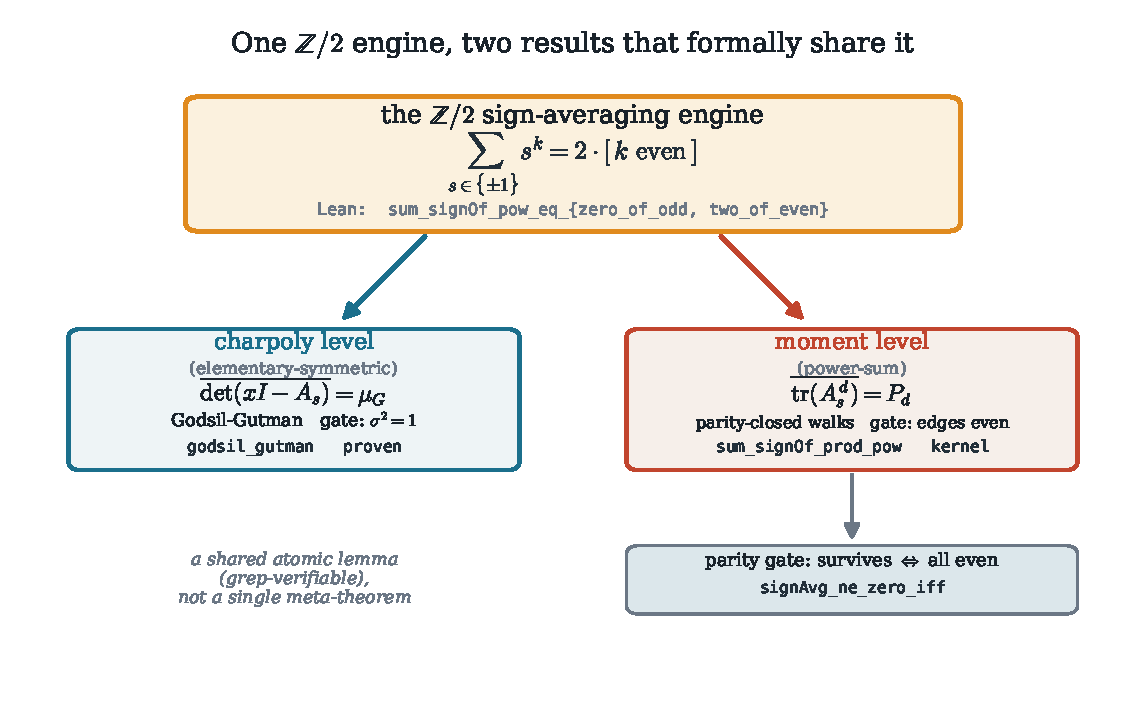
\includegraphics[width=0.92\textwidth]{fig3_zmod2_principle.pdf}
  \caption{One $\Z/2$ sign-averaging fact (\lean{sum\_signOf\_pow}) feeds both
  Godsil--Gutman (characteristic-polynomial level) and the parity-closed-walk
  kernel (moment level). The unification is a shared atomic lemma, visible in
  the dependency graph---not a single meta-theorem; the parity gate
  (\lean{signAvg\_ne\_zero\_iff}) is itself downstream of the moment kernel.}
  \label{fig:engine}
\end{figure}

Here is the part I find genuinely pleasant, and I state it carefully to avoid
over-claiming. The very same per-edge lemmas drive a \emph{second}, seemingly
unrelated identity. Chen, van~Dam and Bu~\cite{ChenVanDamBu2023} observe that the
average $d$-th spectral moment of a signed graph counts its \emph{parity-closed
walks} (closed walks using each edge an even number of times). At the level of
elementary symmetric functions one gets Godsil--Gutman; at the level of power
sums one gets the parity-closed-walk count. They are two readings of the same
$\Z/2$ projection. I formalize the algebraic kernel of the second identity
(\lean{sum\_signOf\_prod\_pow})---its full walk-count form needs walk
infrastructure Mathlib lacks, which I do not claim.

\paragraph{A point of intellectual honesty.}
The unification here is real but modest, and I describe it exactly. I did
\emph{not} prove a single meta-theorem of which both results are corollaries.
What is true---and formally checkable by name---is that both proofs invoke the
\emph{same} atomic lemmas \lean{sum\_signOf\_pow\_eq\_*}. The shared structure
lives in the dependency graph, not in a grand statement, and
Figure~\ref{fig:engine} draws it that way.

% ---------------------------------------------------------------
\section{The bridge to Ramanujan: $2$-lifts}
\label{sec:twolift}

What does any of this have to do with expanders? The link is the $2$-lift.
A signing $s$ of $G$ determines a double cover $G_s$ whose adjacency matrix has
the block form $\bigl[\begin{smallmatrix}A_+&A_-\\A_-&A_+\end{smallmatrix}\bigr]$,
with $A_+,A_-$ the positive- and negative-edge parts. I formalize the
spectral decomposition of this block matrix (\lean{charpoly\_twoLift}):
\[
  \boxed{\;\det\!\Bigl(xI-\begin{bmatrix}B&C\\ C&B\end{bmatrix}\Bigr)
  \;=\;\det(xI-(B{+}C))\cdot\det(xI-(B{-}C))\;},
\]
proved by conjugating with the involution
$\bigl[\begin{smallmatrix}1&1\\1&-1\end{smallmatrix}\bigr]$ (which squares to
$2I$) into block-diagonal form. With $B{+}C=A$ the ordinary adjacency and
$B{-}C=A_s$ the signed one, this says the lift's spectrum is
$\mathrm{spec}(A)\uplus\mathrm{spec}(A_s)$: the \emph{new} eigenvalues are
exactly those of the signed adjacency matrix. So Godsil--Gutman is the
statement that their average characteristic polynomial is $\mu_G$---and
Heilmann--Lieb is the statement that $\mu_G$'s roots respect the Ramanujan
threshold.

I am careful to say what I formalized: the \emph{linear algebra} of the
$2$-lift (the matrix identity above), not the graph-theoretic $2$-lift
construction. That is the right building block, but it is a matrix theorem with
a graph reading, and I present it as such.

% ---------------------------------------------------------------
\section{How the story ends, and where I stopped}
\label{sec:future}

It would be dishonest to pretend I reached the end. I did not. But I can map
it precisely, because the catalog of what remains is short and the route is
classical.
\begin{enumerate}\itemsep2pt
\item[$\checkmark$] Godsil--Gutman (average charpoly $=\mu_G$).
\item[$\checkmark$] The $2$-lift bridge (new eigenvalues $=$ signed eigenvalues).
\item[$\checkmark$] The $\Z/2$ engine tying the spectral and combinatorial sides.
\item[$\circ$] \textbf{Heilmann--Lieb}: $\mathrm{roots}(\mu_G)\subseteq
  [-2\sqrt{\Delta-1},2\sqrt{\Delta-1}]$. The clean route is Godsil's path-tree:
  $\mu_G$ divides the matching polynomial of the path-tree $T(G,u)$; $T$ is a
  forest, on which the matching polynomial \emph{equals} the characteristic
  polynomial (signs are gauge-trivial), hence is real-rooted with the tree
  spectral-radius bound $2\sqrt{\Delta-1}$. This yields real-rootedness and the
  bound in one stroke, and needs no external interlacing machinery.
\item[$\circ$] \textbf{Interlacing families}~\cite{MSS2015a}: the family
  $\{\det(xI-A_s)\}_s$ is interlacing, so some member's largest root is at most
  the largest root of the average $\mu_G$, which is $\le2\sqrt{\Delta-1}$.
\item[$\circ$] Hence a Ramanujan $2$-lift exists, and Ramanujan graphs of every
  degree follow by iterating.
\end{enumerate}
Steps~4--6 are a multi-month undertaking; a literature check (Mathlib plus a web
survey) found no prior formalization of Heilmann--Lieb or of the matching
polynomial in any prover, so the road is unworn but also unbuilt. I think the
honest contribution of this paper is to have laid, and verified, the first few
paving stones, and to have drawn the rest of the map to scale.

% ---------------------------------------------------------------
\section{The next stone: a path-tree proposal}
\label{sec:proposal}

The map in Section~\ref{sec:future} names two unbuilt steps. They are not equal
in cost, and conflating them would be a disservice to anyone deciding what to do
next. So I ask the sharper question:

\begin{quote}\itshape
  what is the \emph{smallest} next step that converts a piece of the map into
  actual road---and how much road does it buy?
\end{quote}

My answer is Heilmann--Lieb via Godsil's \emph{path-tree}, and I think it is a
strikingly good bargain: a single classical construction that delivers both
real-rootedness and the Ramanujan bound at once, with no interlacing machinery.
Here is the plan, in enough detail to start.

\paragraph{The construction.}
Fix a vertex $u$ of $G$. Godsil's path-tree $T(G,u)$ is the tree whose vertices
are the paths in $G$ starting at $u$, with one path joined to another when it
extends it by a single edge (Figure~\ref{fig:pathtree}). It is a finite forest,
and it carries the whole proof on two facts.

\begin{figure}[t]
  \centering
  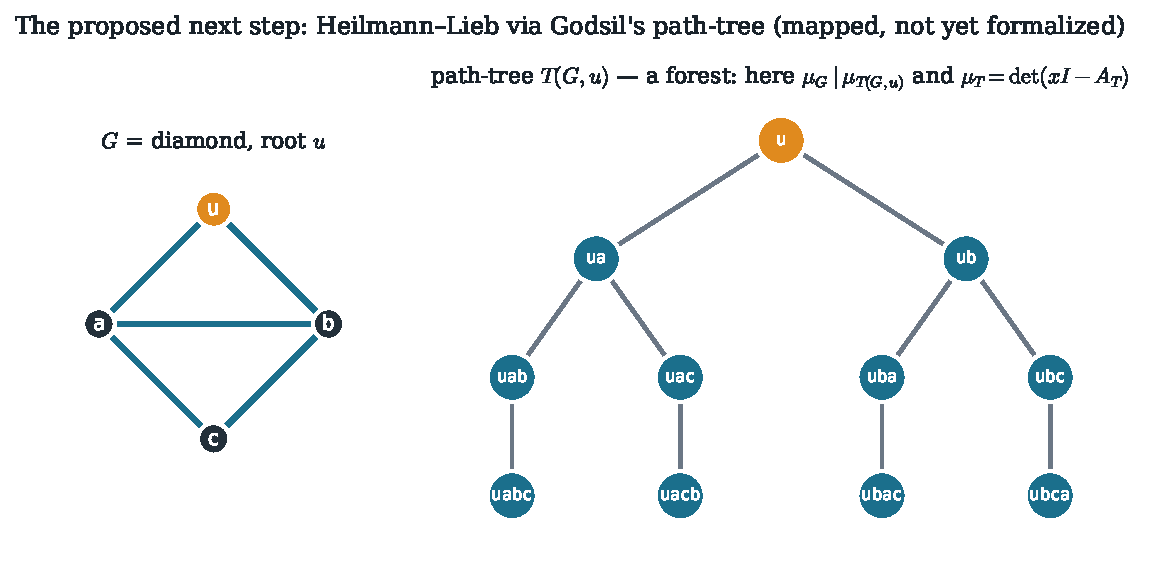
\includegraphics[width=\textwidth]{fig4_path_tree.pdf}
  \caption{Godsil's path-tree $T(G,u)$ of the diamond $G$ (root $u$, amber): its
  vertices are the paths of $G$ starting at $u$, joined when one extends the
  other by an edge. $T(G,u)$ is a forest, so on it the matching polynomial
  \emph{equals} the characteristic polynomial of the adjacency matrix; and
  $\mu_G$ divides $\mu_{T(G,u)}$. These two facts deliver Heilmann--Lieb. The
  construction is mapped here, not yet formalized.}
  \label{fig:pathtree}
\end{figure}

\paragraph{The two facts that do the work.}
\begin{enumerate}\itemsep2pt
\item[(i)] \textbf{Divisibility.} $\mu_G(x)$ divides $\mu_{T(G,u)}(x)$ (Godsil).
  The matching polynomial of the path-tree is a multiple of the one we care
  about, so any root bound for $T$ transfers to $G$.
\item[(ii)] \textbf{Forests are gauge-trivial.} On a forest the matching
  polynomial \emph{equals} the characteristic polynomial of the adjacency
  matrix: a tree has no even cycles to obstruct a global sign change, so signs
  can be gauged away. Hence $\mu_{T(G,u)}$ is the characteristic polynomial of a
  real symmetric matrix, therefore real-rooted; and the spectral radius of a
  tree of maximum degree $\Delta$ is at most $2\sqrt{\Delta-1}$.
\end{enumerate}
Put (i) and (ii) together and $\mu_G$ is real-rooted with all roots in
$[-2\sqrt{\Delta-1},\,2\sqrt{\Delta-1}]$---Heilmann--Lieb, the Ramanujan
threshold, in one stroke. This is why the path-tree is the right stone and not
just \emph{a} stone: it collapses two separate-looking analytic claims into one
combinatorial construction plus standard spectral facts Mathlib already has.

\paragraph{What is already in hand, and what is missing.}
The matching polynomial and its deletion recurrence---the engine of every
path-tree induction---are exactly what this paper formalizes, so the proposal
does not start from zero. What Mathlib still lacks, and what a follow-up must
build, is: the path-tree construction itself (as a \lean{SimpleGraph} on a path
type); the divisibility lemma~(i), whose textbook proof is an induction on the
deletion recurrence; and the forest identity~(ii). I flag one concrete
friction I already met and that this step will meet again: the matching-number
recurrence has a boundary case ($m_N$ of a graph after deleting two adjacent
vertices vanishes) that needs a small isolated-vertices lemma to discharge
cleanly---minor, but the kind of detail a formalization cannot wave away.

\paragraph{An open invitation.}
I state this as a proposal, not a result: none of (i), (ii), or the path-tree
itself is yet formalized, and I do not claim them. But the route is classical,
the prerequisites are now in place, and the payoff---the first machine-checked
Heilmann--Lieb---is well defined. If this paper has a sequel, this is its first
sentence.

% ---------------------------------------------------------------
\section{Implications}
\label{sec:implications}

What might this small piece of work be good for? I list three kinds of
implication, in decreasing order of how confidently I can claim them, and a
methodological aside.

\paragraph{Reusable, certified building blocks.}
The matching polynomial, its deletion recurrence, the signed adjacency matrix,
and the $2$-lift characteristic-polynomial factorization are now
machine-checked and available to anyone working on matchings or signed-graph
spectra in a proof assistant; Mathlib had none of them. Concretely, these are
exactly the pieces a future formalization would build on: Heilmann--Lieb via
Godsil's path-tree (Section~\ref{sec:future}) reuses the matching polynomial and
its recurrence directly; the Gallai--Edmonds structure theorem and the
independence polynomial sit on the same combinatorial infrastructure; and the
signed-adjacency average is the precise recipe behind the broader \emph{method
of interlacing polynomials}---the very technique Marcus, Spielman and Srivastava
used to settle the Kadison--Singer problem~\cite{MSS2015b}. The $\Z/2$
sign-averaging lemmas are tiny, but the paper shows they are reusable across two
levels (elementary-symmetric and power-sum), and I expect them to recur wherever
an expected characteristic polynomial over $\pm1$ signs appears. This is the
implication I can state most firmly: a handful of new, certified foundations.

\paragraph{A stepping stone toward formalized Ramanujan existence.}
The Marcus--Spielman--Srivastava theorem---Ramanujan graphs of every
degree---is celebrated, and no proof assistant has yet touched it. This paper
formalizes its structural half and maps the analytic half
(Section~\ref{sec:future}) to scale. Should the landmark ever be built, these
are foundations it can stand on, and the map may spare the next person the
literature survey I had to run.

\paragraph{The mathematics, with a note of caution.}
Ramanujan graphs and expanders are not abstract curiosities: they underpin
error-correcting codes (LDPC and expander codes), derandomization (Reingold's
log-space algorithm for undirected connectivity uses expander walks), fast
Laplacian solvers, cryptographic hash functions built from isogeny/expander
graphs, and robust communication networks---that is why the underlying theorem
matters. I am wary, though, of borrowing that importance for this paper. Formalizing a foundational identity does not by itself ship a code
or a network; its value lies in certified foundations and in the growing corpus
of formalized mathematics, not in immediate application. I claim the former and
not the latter.

\paragraph{A methodological aside.}
This development was carried out with an AI system as a research instrument: it
proposed definitions, lemmas and tactics, and a build-as-oracle loop verified
or rejected each against the kernel. The careful accounting in this paper---
every claim sized to exactly what was proved, the limitations stated as plainly
as the results---is itself part of what I hope the work illustrates: that
AI-assisted formalization can avoid the over-claiming the method invites,
precisely because the proof assistant, not the assistant, has the last word.

% ---------------------------------------------------------------
\section{Related work}
\label{sec:related}

The mathematics is classical: Godsil--Gutman~\cite{GodsilGutman1981},
Heilmann--Lieb~\cite{HeilmannLieb1972}, the Marcus--Spielman--Srivastava
program~\cite{MSS2015a,MSS2015b}, and the $2$-lift / Bilu--Linial picture
underlying it; the moment-level companion is recent~\cite{ChenVanDamBu2023}.
On the formalization side, Mathlib~\cite{Mathlib2020} provides simple graphs and
characteristic polynomials but neither the matching polynomial nor signed-graph
spectral theory. The development sits in a growing line of Lean combinatorics
formalizations---Hall's marriage theorem~\cite{GusakovMehtaMiller2021}, the
Kruskal--Katona theorem~\cite{Mehta2022KruskalKatona}, Szemer\'edi's regularity
lemma~\cite{DilliesMehta2022}, and proof pearls in the same
spirit~\cite{Mehta2023Sharkovsky}---none of which touches matching polynomials or
signed-graph spectra. The interlacing toolkit of PerAlexandersson's
\texttt{RealRooted} is a research codebase, not a polished library, and does not
include the matching polynomial; my planned path-tree route
(Section~\ref{sec:proposal}) sidesteps it.
I am not aware of any prior machine-checked treatment of these results.

% ---------------------------------------------------------------
\section{Conclusion}

I set out from a simple question---what is the average characteristic
polynomial of a random signing?---and followed it, in a proof assistant, to a
complete and checked answer (Godsil--Gutman), to the small $\Z/2$ fact that
makes it tick, to a second identity that shares that fact, and to the matrix
bridge that points it all at Ramanujan graphs. None of these results is new
mathematics; the contribution is that they are now machine-verified, that the
matching polynomial exists in a prover for the first time, and that the shared
engine is visible in the dependency graph rather than asserted. The deep half
of the story---Heilmann--Lieb and interlacing families---remains ahead of me,
mapped but unbuilt. I offer this as a pearl and an invitation.

\paragraph{Artifacts.} All Lean sources (\lean{sorry}-free; \lean{\#print
axioms} reporting only \lean{propext}, \lean{Classical.choice},
\lean{Quot.sound}), the figures of this paper, and the numerical cross-checks of
Table~\ref{tab:checks} are available at
\url{https://github.com/karlesmarin/godsil-gutman-lean}.

\bibliographystyle{plain}
\bibliography{references}

\end{document}
